\section{ネットワークの変更}
春山らの先行研究では,~~に示すネットワークを使用していた.
一方でfelipeらの先行研究によると,~~に示す,モデルがコマンドによって分岐する形式のネットワークがより経路追従の成功率が向上すると報告している.
そのため,今回の研究ではfelipeらによって提案されたネットワークを参考に新たなネットワークを構築した.

\begin{figure}[htbp]
  \centering
   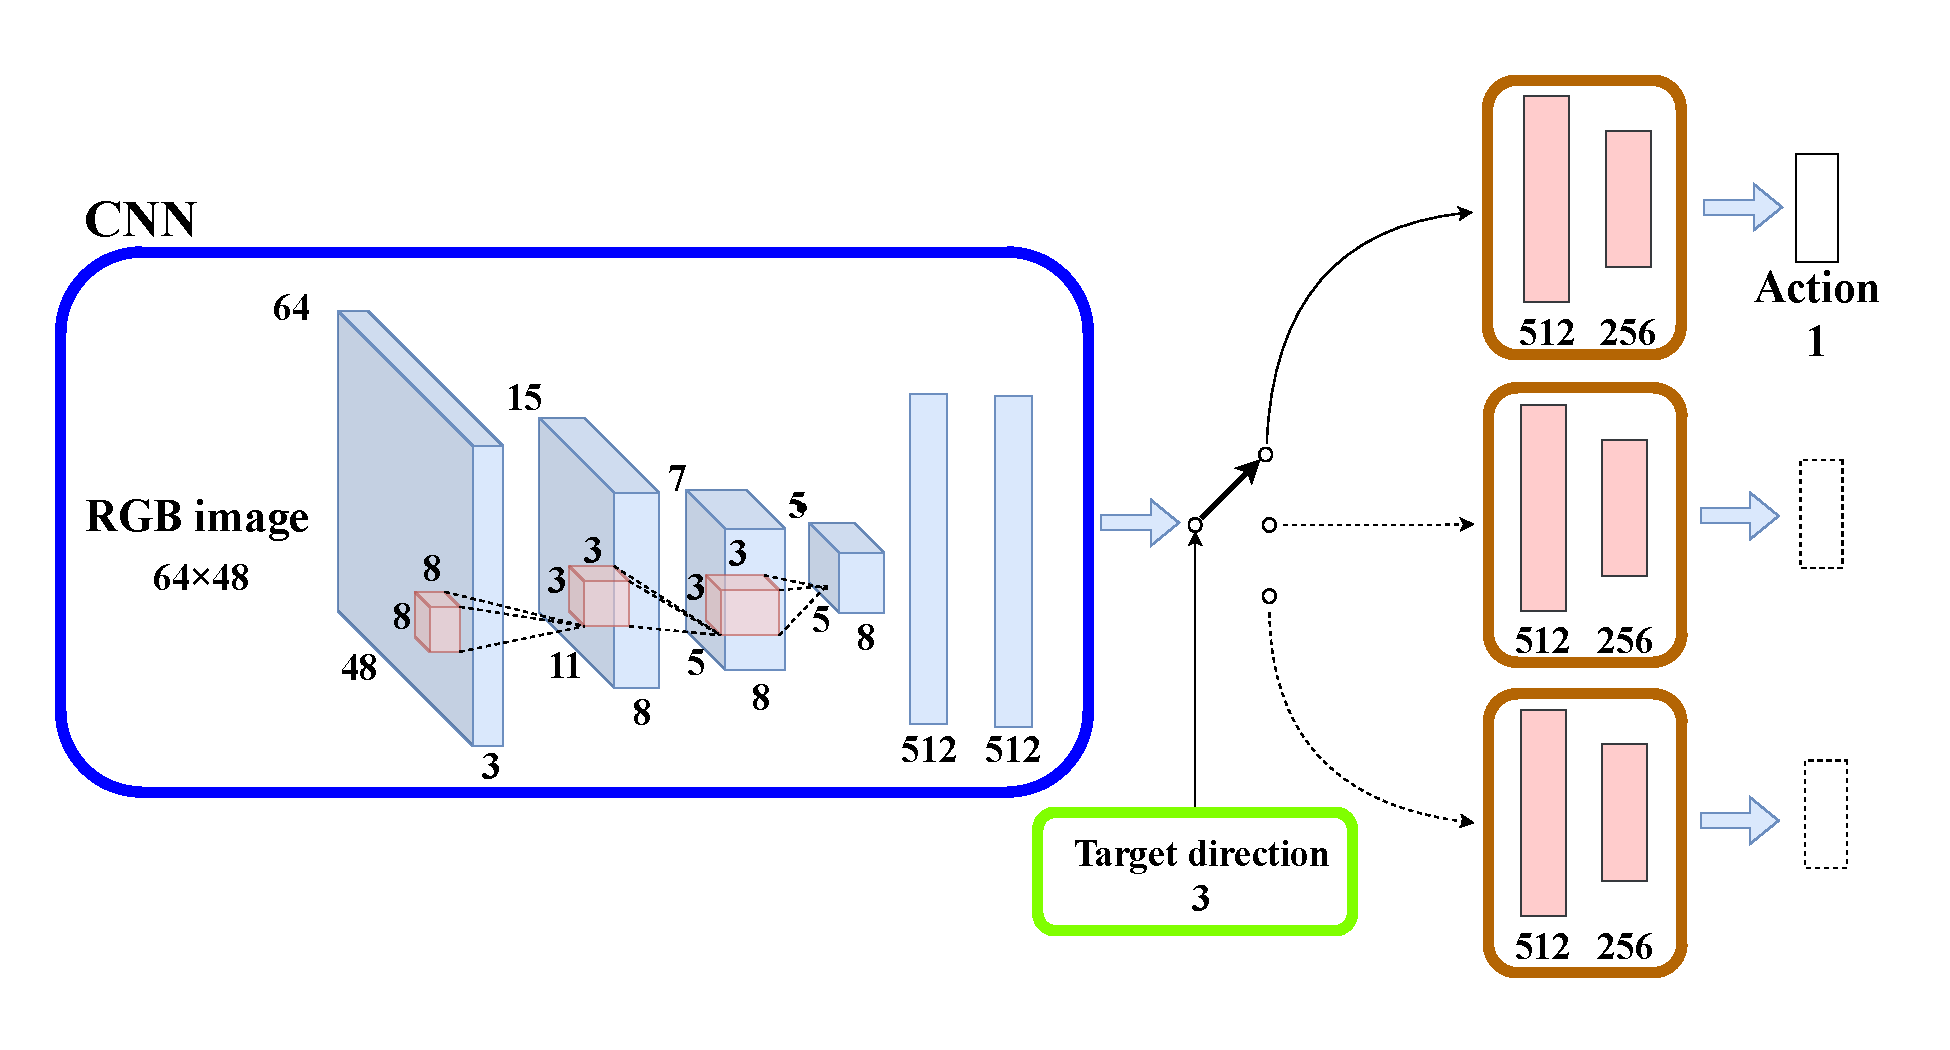
\includegraphics[width=130mm]{images/pdf/ishiguro/branched.pdf}
   \caption{Branched network}
   \label{fig:branched}
\end{figure}